% mnras_template.tex 
%
% LaTeX template for creating an MNRAS paper
%
% v3.0 released 14 May 2015
% (version numbers match those of mnras.cls)
%
% Copyright (C) Royal Astronomical Society 2015
% Authors:
% Keith T. Smith (Royal Astronomical Society)

% Change log
%
% v3.0 May 2015
%    Renamed to match the new package name
%    Version number matches mnras.cls
%    A few minor tweaks to wording
% v1.0 September 2013
%    Beta testing only - never publicly released
%    First version: a simple (ish) template for creating an MNRAS paper

%%%%%%%%%%%%%%%%%%%%%%%%%%%%%%%%%%%%%%%%%%%%%%%%%%
% Basic setup. Most papers should leave these options alone.
\documentclass[fleqn,usenatbib]{mnras}

% MNRAS is set in Times font. If you don't have this installed (most LaTeX
% installations will be fine) or prefer the old Computer Modern fonts, comment
% out the following line
\usepackage{newtxtext,newtxmath}
% Depending on your LaTeX fonts installation, you might get better results with one of these:
%\usepackage{mathptmx}
%\usepackage{txfonts}

% Use vector fonts, so it zooms properly in on-screen viewing software
% Don't change these lines unless you know what you are doing
\usepackage[T1]{fontenc}
\usepackage{ae,aecompl}


%%%%% AUTHORS - PLACE YOUR OWN PACKAGES HERE %%%%%

% Only include extra packages if you really need them. Common packages are:
\usepackage{graphicx}	% Including figure files
\usepackage{amsmath}	% Advanced maths commands
\usepackage{amssymb}	% Extra maths symbols

%%%%%%%%%%%%%%%%%%%%%%%%%%%%%%%%%%%%%%%%%%%%%%%%%%

%%%%% AUTHORS - PLACE YOUR OWN COMMANDS HERE %%%%%

% Please keep new commands to a minimum, and use \newcommand not \def to avoid
% overwriting existing commands. Example:
%\newcommand{\pcm}{\,cm$^{-2}$}	% per cm-squared
\newcommand{\red}[1]{{\textcolor{red}{#1}}}
\newcommand{\green}[1]{{\textcolor{green}{#1}}}
\newcommand{\blue}[1]{{\textcolor{blue}{#1}}}

%%%%%%%%%%%%%%%%%%%%%%%%%%%%%%%%%%%%%%%%%%%%%%%%%%

%%%%%%%%%%%%%%%%%%% TITLE PAGE %%%%%%%%%%%%%%%%%%%

% Title of the paper, and the short title which is used in the headers.
% Keep the title short and informative.
\title[Decoupling star-gas rotation - II]{Decoupling star-gas rotation - II: black hole luminosity and feedback in counter-rotating low mass galaxies}

% The list of authors, and the short list which is used in the headers.
% If you need two or more lines of authors, add an extra line using \newauthor
\author[C. Duckworth et al.]{Christopher Duckworth,$^{1,2}$\thanks{E-mail: cd201@st-andrews.ac.uk}
et al.
\\
% List of institutions
$^{1}$School of Physics and Astronomy, University of St Andrews, North Haugh, St Andrews, KY16 9SS, UK\\
$^{2}$Center for Computational Astrophysics, Flatiron Institute, 162 Fifth Avenue, New York, NY 10010, USA\\
}

% These dates will be filled out by the publisher
\date{Accepted XXX. Received YYY; in original form ZZZ}

% Enter the current year, for the copyright statements etc.
\pubyear{2019}

% Don't change these lines
\begin{document}
\label{firstpage}
\pagerange{\pageref{firstpage}--\pageref{lastpage}}
\maketitle

% Abstract of the paper
\begin{abstract}

\end{abstract}

% Select between one and six entries from the list of approved keywords.
% Don't make up new ones.
\begin{keywords}
keyword1 -- keyword2 -- keyword3
\end{keywords}

%%%%%%%%%%%%%%%%%%%%%%%%%%%%%%%%%%%%%%%%%%%%%%%%%%

%%%%%%%%%%%%%%%%% BODY OF PAPER %%%%%%%%%%%%%%%%%%

\section{Introduction}
Tidal torque theory \citep[TTT;][]{hoyle1951, peebles1969, Doroshkevich1970} dictates that the angular momentum content of collapsing baryons are inherited from the surrounding dark matter halo. In the framework of a $\Lambda$ cold dark matter ($\Lambda$CDM) Universe, galaxies form from the cooling and condensation of the initial gas cloud within dark matter haloes \citep{fall1980, mo1998}. As stars form from the rotating gas, a natural expectation is that they will inherit its dynamical characteristics leading to coherent rotation between dark matter, gas and stars in both magnitude and direction. However, after turnaround there is good reason to believe that the rotation of dark matter, gas and stars may decouple from each other as galaxies evolve up-to $z=0$. 

Recent sophisticated cosmological scale hydro-dynamical simulations have provided a clear insight into the nature of the relationship between the angular momentum of baryons and dark matter through cosmic time. A necessary component of realistic simulations is efficient feedback from both black holes (BH) and stars, required to, amongst other things, reproduce late type disks and solve the problem of catastrophic angular momentum loss \citep[e.g.][]{zavala2008, scannapieco2009}. Active galactic nuclei (AGN) and supernova explosions can also lead to dramatic redistribution of gas. Galactic winds carry both mass and angular momentum leading to potential boosts in angular momentum \citep[e.g.][]{DeFelippis2017}. 

The ability of black holes to disrupt angular momentum can depend on the `mode' of feedback. `Quasar' (radiative) mode feedback releases huge amounts of energy through radiation from the accretion disk leading to high luminosity AGN and dramatic gas outflow and loss \citep[e.g.][]{cattaneo2009, rubin2014, cheung2016}. Alternatively `radio' mode is termed for lower luminosity AGN that host lower black hole accretion rates. In this instance energy is deposited into the surrounding gas via jets and winds which heat the gas and suppress star formation \citep[][]{binney1995, ciotti2001, heckman2014}.

Understanding how exactly AGN relate to stellar and gas kinematics have been the focus of several recent studies using Integral Field Spectroscopy (IFS) data. In particular, a new class of galaxy termed `red geyser' has been identified which hosts AGN and exhibits with high velocity outflows in the spatial distribution of ionized gas \citep[][]{cheung2016, roy2018}. These outflows are often linked to a distinctive offset in rotation direction between the stars and gas. It is estimated that approximately $5-10$\% of the quiescent population currently exhibit these outflows. \citet{penny2018} demonstrate the importance of AGN feedback in low mass quiescent galaxies. While the majority demonstrate no ionized gas present, quiescent galaxies with an active AGN that is actively suppressing star formation show a clear decoupling in the rotation of stars and gas. 

Despite this, the relationship to the kinematics of stars and ionized gas is not clear for all galaxies with identified AGN. \citet{ilha2019} find that typical rotation offsets between stars and gas in AGN defined galaxies are consistent with inactive controls. Termed kinematic misalignment, the decoupled rotation of stars and gas can also be a natural result of external processes \cite[e.g.][]{davis2011, barrera2015, vdvoort2015, chen2016, jin2016, starkenburg+19}.

%Regardless of internal or external origin, kinematic misalignment is linked with both typical lower gas mass fractions and angular momentum \citep[e.g. Duckworth et al. submitted,][]{starkenburg+19}. 

Recent studies have shown a strong relationship between visual morphology and the likelihood of misalignment \citep[e.g. Duckworth et al. submitted,][]{chen2016, bryant2019}. Properties such as stellar mass are different when comparing aligned and misaligned galaxies of the same morphology and the difference (whether positive or negative) is morphologically dependent. Misaligned early-type galaxies are more massive, whereas misaligned late-types are less massive when compared to their aligned controls. This could be an indication that whether the misalignment is internally or externally driven is also morphologically dependent. \red{not sure about this motivation. maybe need to talk about low mass galaxies more}

Given the ubiquity of misalignment in quiescent AGN bright galaxies, a natural question arises; \textit{do we expect a correlation in AGN luminosity and misalignment for all galaxies?} In this letter, we study the relationship between black hole feedback, black hole luminosity and kinematic misalignment in the cosmological scale hydrodynamical simulation of IllustrisTNG (TNG). We use a MaNGA like sample defined in TNG to emulate what we may expect to see in IFS observations in terms of morphological dependence and correlation timescales. In Section \ref{sec:methods} we briefly describe the simulation and how we construct our sample. In Section \ref{sec:results} we present our results before concluding in Section \ref{sec:conclusion}.

\section{Methods} \label{sec:methods}
For this work, we use the fiducial run of IllustrisTNG-100 (hereafter referred to as TNG) which follows the evolution of 2 x 1820$^3$ resolution elements within a periodic cube with box lengths of 110.7 Mpc (75 h$^{-1}$ Mpc). This corresponds to an average mass resolution of baryonic elements of 1.4 x 10$^6 M_{\odot}$ and 7.5 x 10$^6 M_{\odot}$ for dark matter. The IllustrisTNG project \citep{marinacci18,naiman18,nelson18,pillepich18b,springel18} is a suite of magneto-hydrodynamic cosmological scale simulations incorporating an updated comprehensive model for galaxy formation physics \citep[as decribed in; ][]{weinberger17,pillepich18a} and making use of the moving-mesh code \texttt{AREPO} \citep{springel10,pakmor11,pakmor13}. 

Of particular relevance to this study is the the prescription of \citet{weinberger17} for AGN feedback. As in other hydrodynamical cosmological simulations \citep[e.g.][]{dubois2016}, AGN feedback is modelled by two modes (quasar mode: high accretion, kinetic mode: low accretion). The transition is dictated by both the BH mass and accretion rate onto the BH, so that as BHs grow over time the kinetic mode is likely to become more dominant. We note that in the kinetic model, the direction of injected momentum is random. 

To emulate what we may expect to see in IFS observations we construct a sample of TNG galaxies with mock MaNGA \citep[Mapping Galaxies at Apache Point;][]{bundy2015, blanton2017} observations. Set to complete in 2020, the MaNGA survey is designed to investigate the internal structure of $\sim$10000 galaxies in the nearby Universe. By design, the complete sample is unbiased towards morphology, inclination and colour and provides a near flat distribution in stellar mass. For each MaNGA galaxy, we find an object in TNG with the closest match in stellar mass, $g-r$ colour and size. We define the degree of misalignment between the rotation of stars and gas by fitting a position angle (PA) to the mock MaNGA velocity fields using the \texttt{fit\_kinematic\_pa} routine \citep[see Appendix C of][for a description of the process]{krajnovic2006} so that $\Delta PA = |PA_{stellar} - PA_{H\alpha}|$. We take objects with $\Delta$PA < 30$^{\circ}$ to be aligned, $\Delta$PA > 30$^{\circ}$ to be misaligned and $\Delta$PA > 150$^{\circ}$ to be counter-rotating. For a complete description of the construction of this sample, mock observations and PA fitting we direct the reader to Duckworth et al. submitted. We use approximately X galaxies with defined $\Delta$PAs in this work. 

\section{Results} \label{sec:results}
Each panel of Figure \ref{fig:overall_pop} shows the time evolution average of a property for all galaxies split by stellar mass (Top 33\% - red, Bottom 33\% - blue) and $\Delta$PA (< 30$^{\circ}$ - solid, > 30$^{\circ}$ - dashed, > 150$^{\circ}$ - dotted) both defined and split at $z=0$. Columns left to right show the evolutions for each of quenched, green valley and star forming galaxies individually \cite[defined by deviation from the star forming main-sequence ][]{pillepich2019}. 

Starting with the top row, we see distinct correlations between $\Delta$PA at $z=0$ and BH luminosity ($log_{10}(L_{bol})$) in the last 8 Gyr for all low mass galaxies. This is most apparent for green valley and star forming galaxies that are found as counter-rotating at $z=0$, however a boost can be seen for all misaligned galaxies. In contrast, we note that the correlation between misalignment and AGN luminosity for the high mass bin is unclear. Since low (high) mass galaxies in TNG exhibit `quasar' (`kinetic') mode feedback, a possible interpretation is that quasar mode feedback is more likely to lead to misaligned gas rotation.

In the second row we plot the gas fraction ($M_{gas}$/$M_{stel}$) for each sample. For all low mass galaxies, gas loss is a key feature, potentially indicative of gas outflows from the feedback. Interestingly, we find that the gas fraction for misaligned high mass quenched galaxies grows with time to eventually become consistent with the aligned value by $z=0$. This is indicative that mass growth from accretion and gas rich minor mergers is potentially more important for decoupling their rotation. Further evidence for this can be found by the gas phase metallicity (Z) in the fourth row. We find that the gas in misaligned high mass quenched galaxies has typically lower metallicity, indicative of more recent accretion.

In the third row we show the time evolution of specific angular momentum for all gas within a 3D radius of the IFS observational footprint (typically 1.5-2.5 effective radii). For all misaligned galaxies, regardless of the misalignment mechanism, we see a common theme that specific angular momentum of gas decays as time approaches $z=0$. \red{not sure this adds anything to argument I am trying to make..}

In the fourth row we see that gas phase metallicity is often boosted in the last 4 Gyr for low mass galaxies exhibiting misalignment. This appears to correlate with gas fraction showing that... A) feedback triggers metallicity increase? B) feedback blows out pristine gas?

Finally in the bottom row, we plot the specific star formation rate (sSFR) for all gas cells in the galaxy. We find that, in general, sSFR is decreased for low mass misaligned galaxies, indicative that the BH feedback is actively suppressing star formation as it drives gas out of the galaxies. \red{why do we see suppressed star formation for the massive ETGs if they are acquiring gas - is kinetic feedback displacing gas but not removing it? - is the acquired gas too hot to form stars?}

\begin{figure*}
	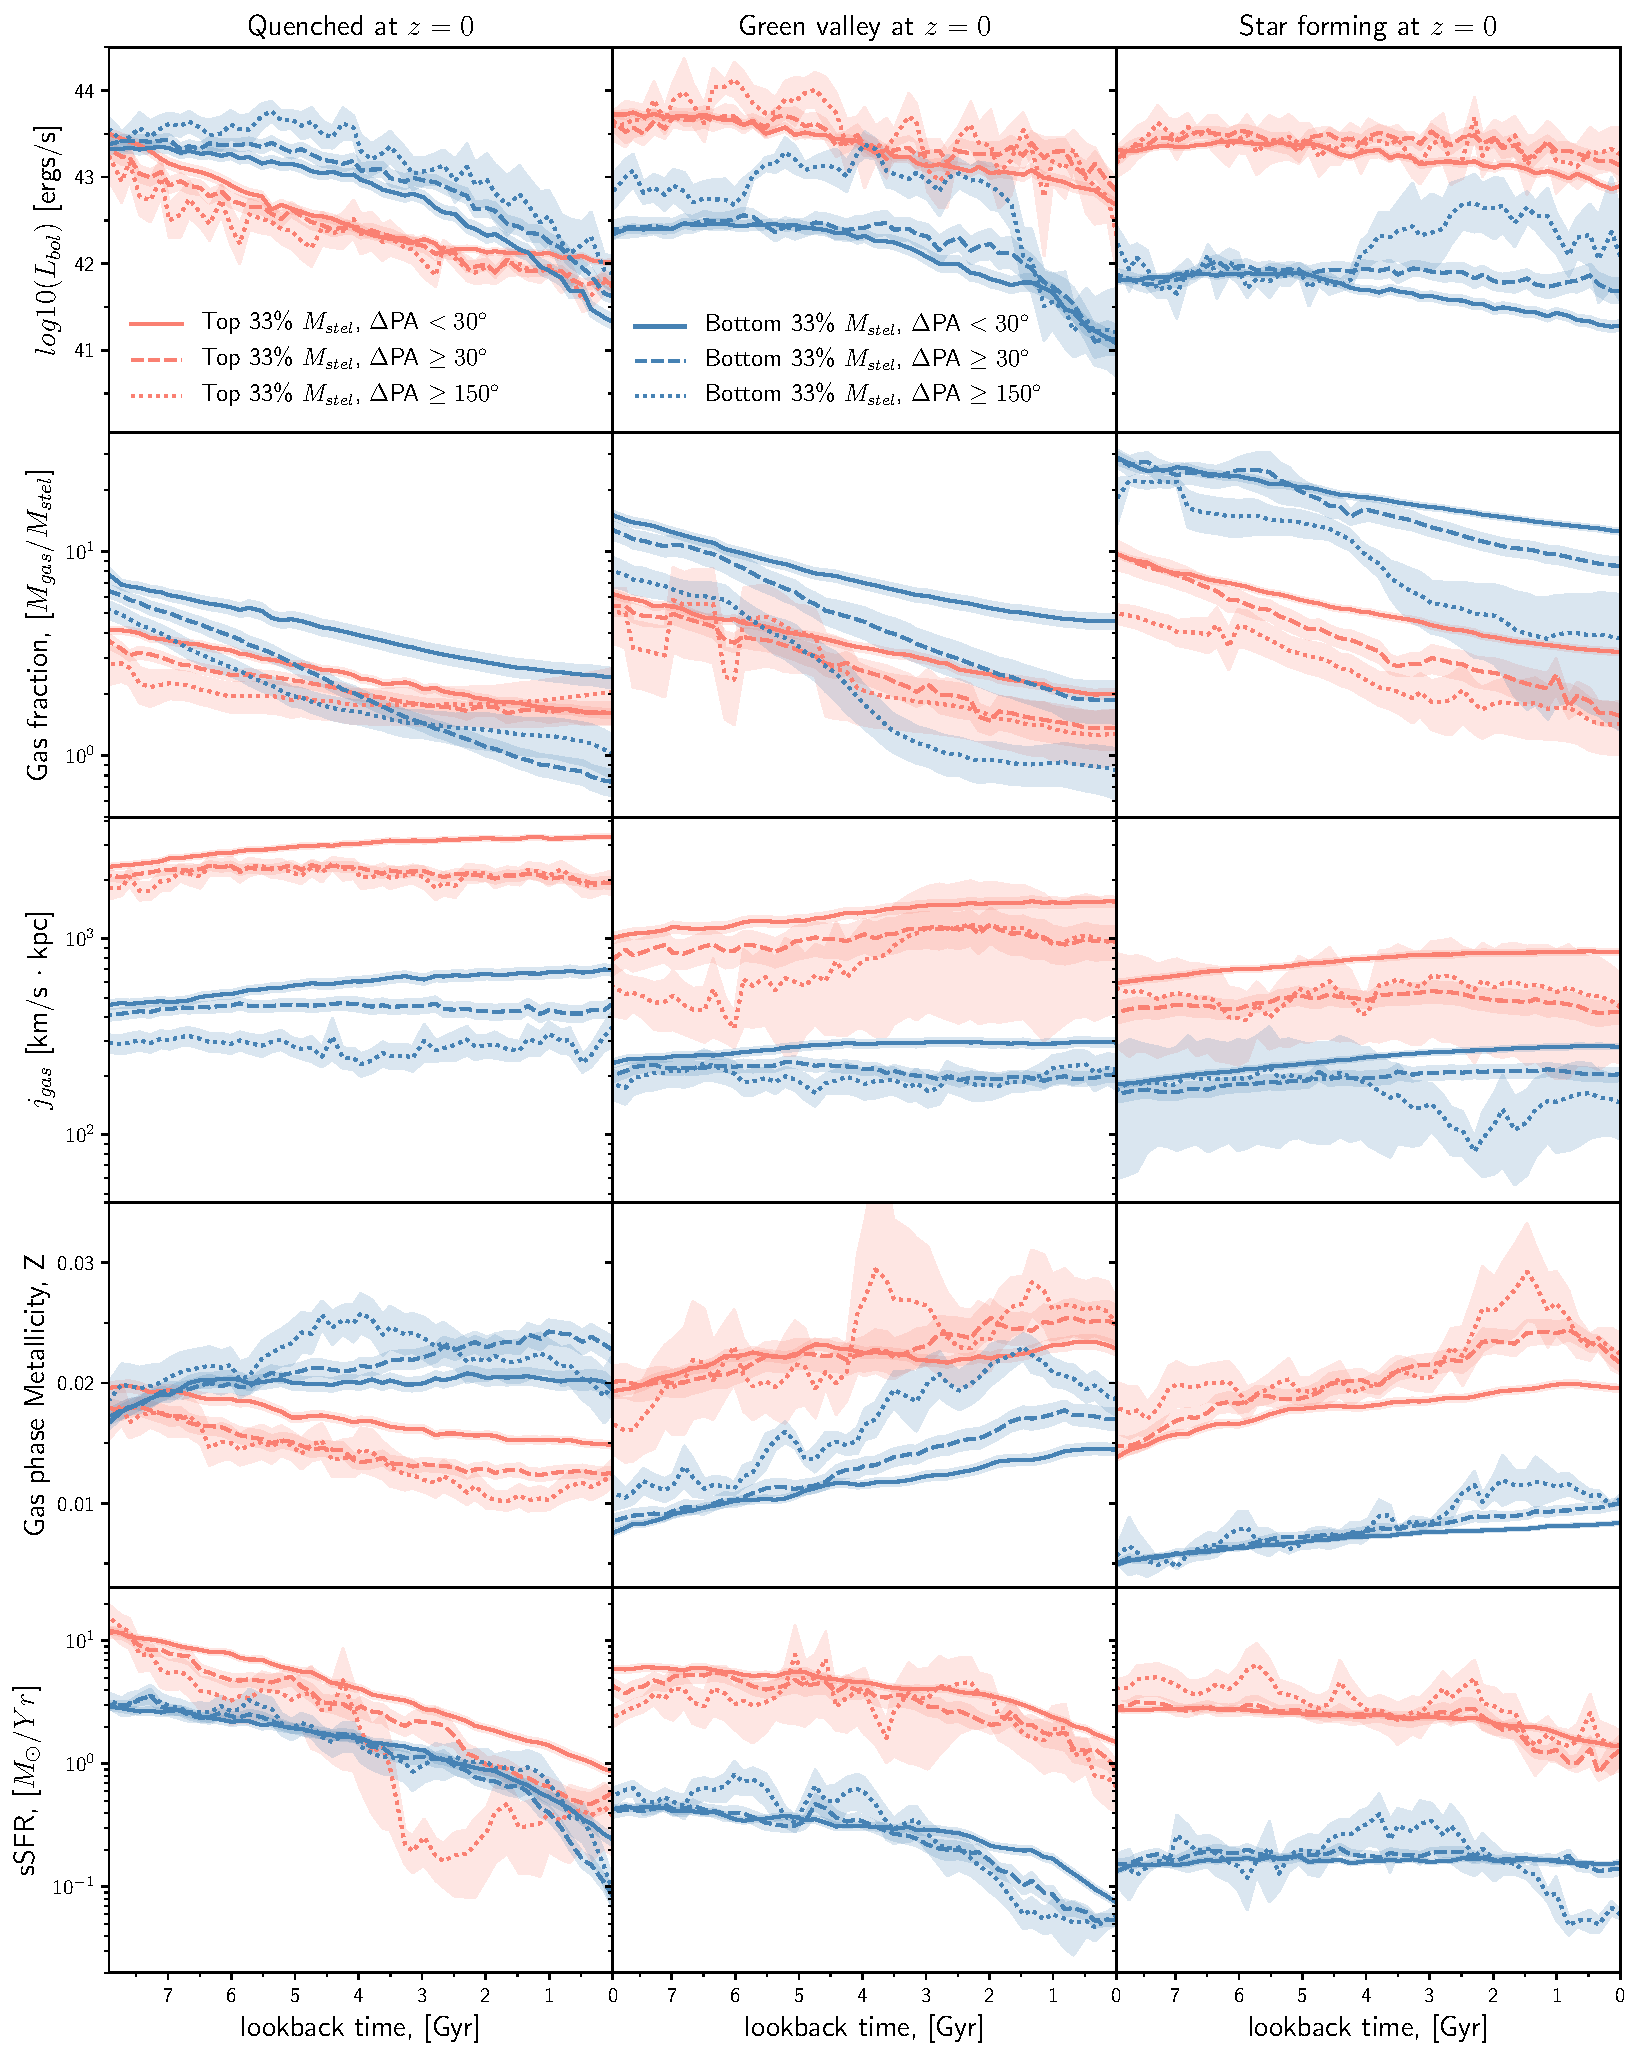
\includegraphics[width=0.9\linewidth]{overall_population/overall_pop_evolution.pdf}
    \caption{Time evolution of (rows top to bottom) black hole luminosity ($log_{10}(L_{bol})$), gas fraction ($M_{gas}$/$M_{stel}$), gas angular momentum ($j_{gas}$), gas phase metallicity and specific star formation rate for (columnns left to right) quenched, green valley and star forming galaxies identified at $z=0$. In each panel, the time evolution is split into the top 33\% (red) and bottom 33\% (blue) in stellar mass and also $\Delta$PA $< 30^{\circ}$ (solid) and $> 30^{\circ}$ (dashed) and  $> 30^{\circ}$ (dotted). Each line shows the mean for the population with the shaded region corresponding to the standard error.}
    \label{fig:overall_pop}
\end{figure*}

To better understand the relationship between misalignment and BH feedback in low mass galaxies, in Figure \ref{fig:LM_BH} we show the time evolution of energy injection into the surrounding gas cells and black hole mass. For these properties we plot the average residual difference of misaligned (dashed) and counter-rotating (dotted) galaxies with respect to the aligned galaxies (grey dashed line at the origin). We find that the rate of energy injection is richer for low mass counter-rotating galaxies, however a boost can be seen for all those that are misaligned.

Interestingly, as for the BH luminosity, the lookback time at which feedback energy injection peaks appears to be different as a function of morphology. Star forming galaxies show far more recent feedback and BH luminosity, indicative that while the gas is in the process of being decoupled and blown out, it hasn't acted to fully quench the galaxy yet. Conversely, looking at green valley and quenched galaxies we can see that the feedback starts earlier allowing for the drop in SFR we see today.

We also show the residual time evolution of black hole mass with respect to the aligned galaxies. For all low mass galaxies, we see a steady divergence of misaligned galaxies from the aligned control as black hole mass difference increases over time. As we see that angular momentum is disrupted in misaligned galaxies, it may be natural to think that this leads to an increased inflow of gas into the galaxy centre and hence black hole.

\begin{figure*}
	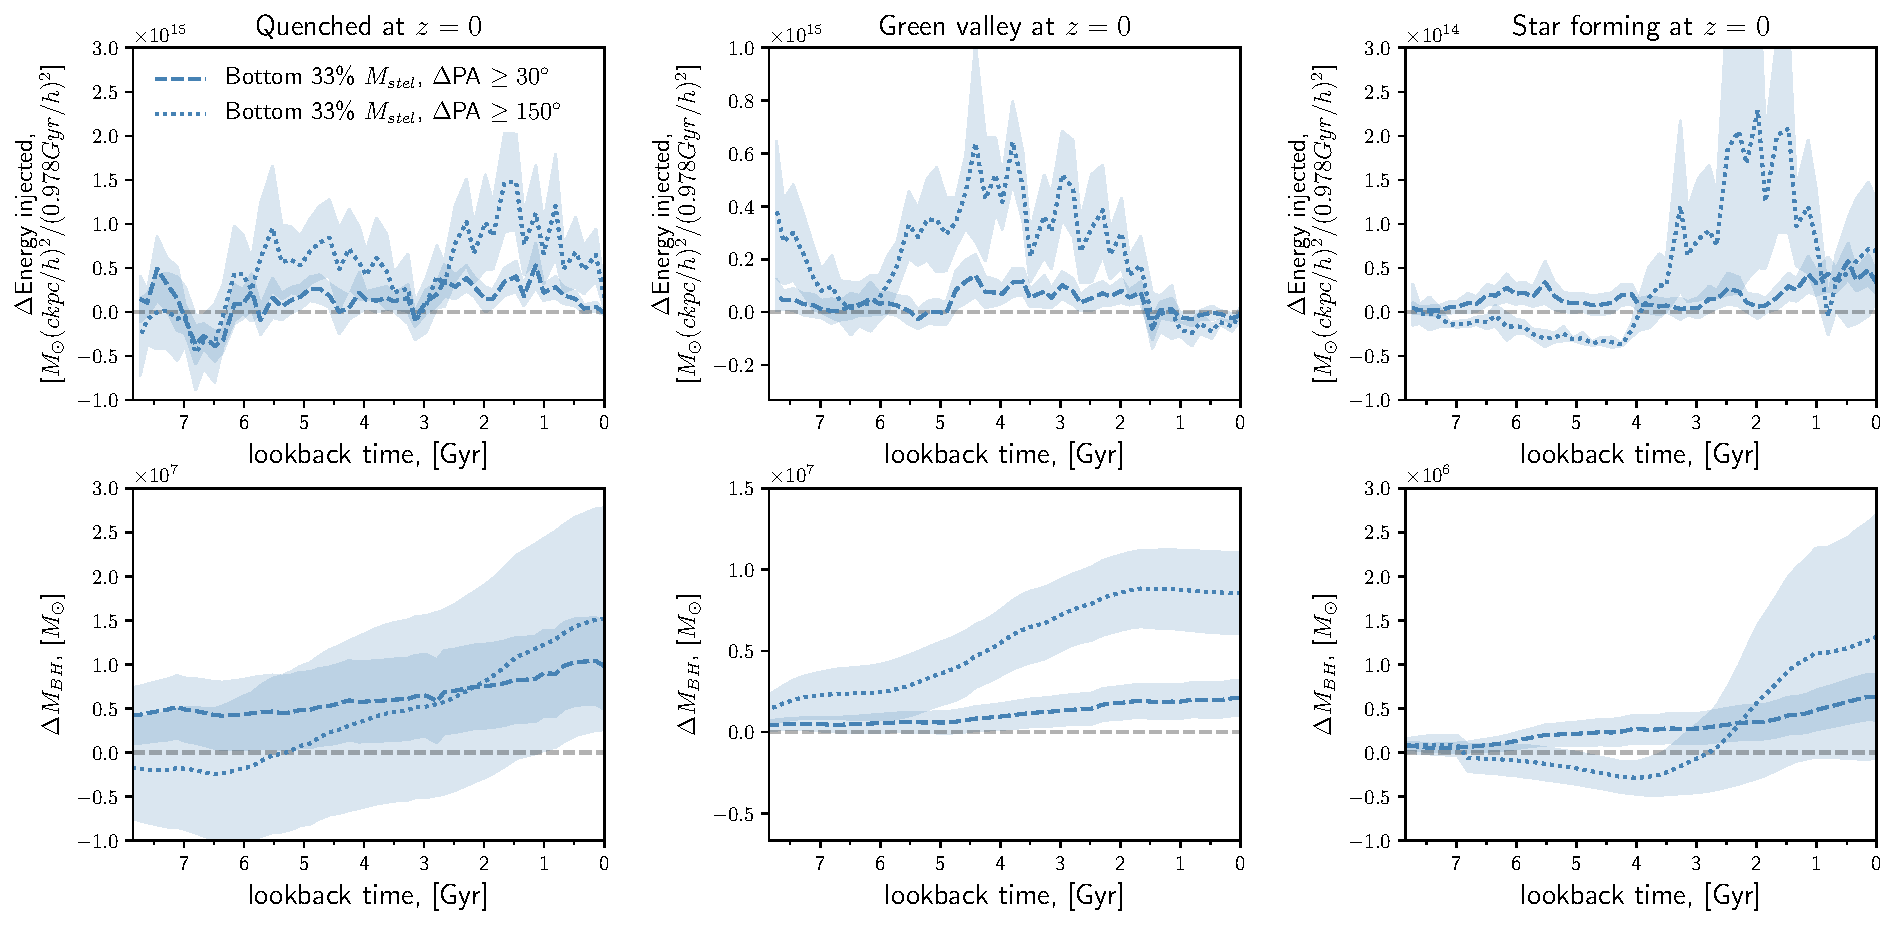
\includegraphics[width=0.9\linewidth]{overall_population/LM_BH_residual_evo.pdf}
    \caption{Time evolution of black hole energy injection (top; see main text for more detail) and black hole mass (bottom) for (columnns left to right) quenched, green valley and star forming galaxies identified at $z=0$. Shown are residuals for the bottom 33\% in stellar mass for $\Delta$PA$ > 30^{\circ}$ (dashed) and $\Delta$PA$ > 150^{\circ}$ (dotted) defined relative to $\Delta$PA$ < 30^{\circ}$. Each line shows the mean for the population with the shaded region corresponding to the standard error.}
    \label{fig:LM_BH}
\end{figure*}

\red{To be included: figure of deltaPA as a function of BH luminosity (for low and high masses?) - to compare to observations. While BH luminosity is correlated with misalignment over timescales, it might not be correlated instantaneously.}

\section{Discussion and Conclusion} \label{sec:conclusion}
Talk about black hole feedback modes in IllustrisTNG; quasar and kinetic modes and hence why this might be seen more in low mass galaxies.

Talk about time dependence of misalignment as function of morphology - this could be why you don't always see AGN composite.

\section*{Acknowledgements}


%%%%%%%%%%%%%%%%%%%%%%%%%%%%%%%%%%%%%%%%%%%%%%%%%%

%%%%%%%%%%%%%%%%%%%% REFERENCES %%%%%%%%%%%%%%%%%%

% The best way to enter references is to use BibTeX:

\bibliographystyle{mnras}
\bibliography{biblio} 

%%%%%%%%%%%%%%%%%%%%%%%%%%%%%%%%%%%%%%%%%%%%%%%%%%

%%%%%%%%%%%%%%%%% APPENDICES %%%%%%%%%%%%%%%%%%%%%

\appendix

\section{Some extra material}

If you want to present additional material which would interrupt the flow of the main paper,
it can be placed in an Appendix which appears after the list of references.

%%%%%%%%%%%%%%%%%%%%%%%%%%%%%%%%%%%%%%%%%%%%%%%%%%


% Don't change these lines
\bsp	% typesetting comment
\label{lastpage}
\end{document}

% End of mnras_template.tex